% TODO:
% Better picture of HC-05?
% Update architecture PNG - ardiunos don't talk to arduinos
% Architecture figure to different section
% 'IoT' or 'Internet of Things'? need to define IoT earlier!
% Mention outreach?
% Sort out topics!
% Ensure that what is written here about Bluetooth working with our setup if a set of devices is provided is correct
% Sort out tenses


We implemented a test bed for future development of an Internet of Things security protocol. Our proof-of-concept uses standard IoT components to produce a system that propagates data over the different levels of our architecture, demonstrating common features of a large scale infrastructure.


% ✔ We wanted to make a prototype for use as a test bed (or proof-of-concept) for future development of an IoT security protocol, blah.
% Also used for outreach activities, blah
% ✔ Chose to use off-the-shelf component for maximum applicability, blah


\subsection{Equipment}

For Edge Devices, we used Arduino Unos which are inexpensive (£25-30), low powered and portable making them a popular choice for use with IoT. With 14 inputs and outputs (analog and digital), these microcontrollers can be loaded with pre-compiled programs to interact with sensors. For communication, we used serial to send and receive data with the Smart Agents. This was wired (over USB) or wireless through the addition of a HC-05 Bluetooth module (see Figure \ref{fig:HC-05}).


\begin{figure}
    \centering
    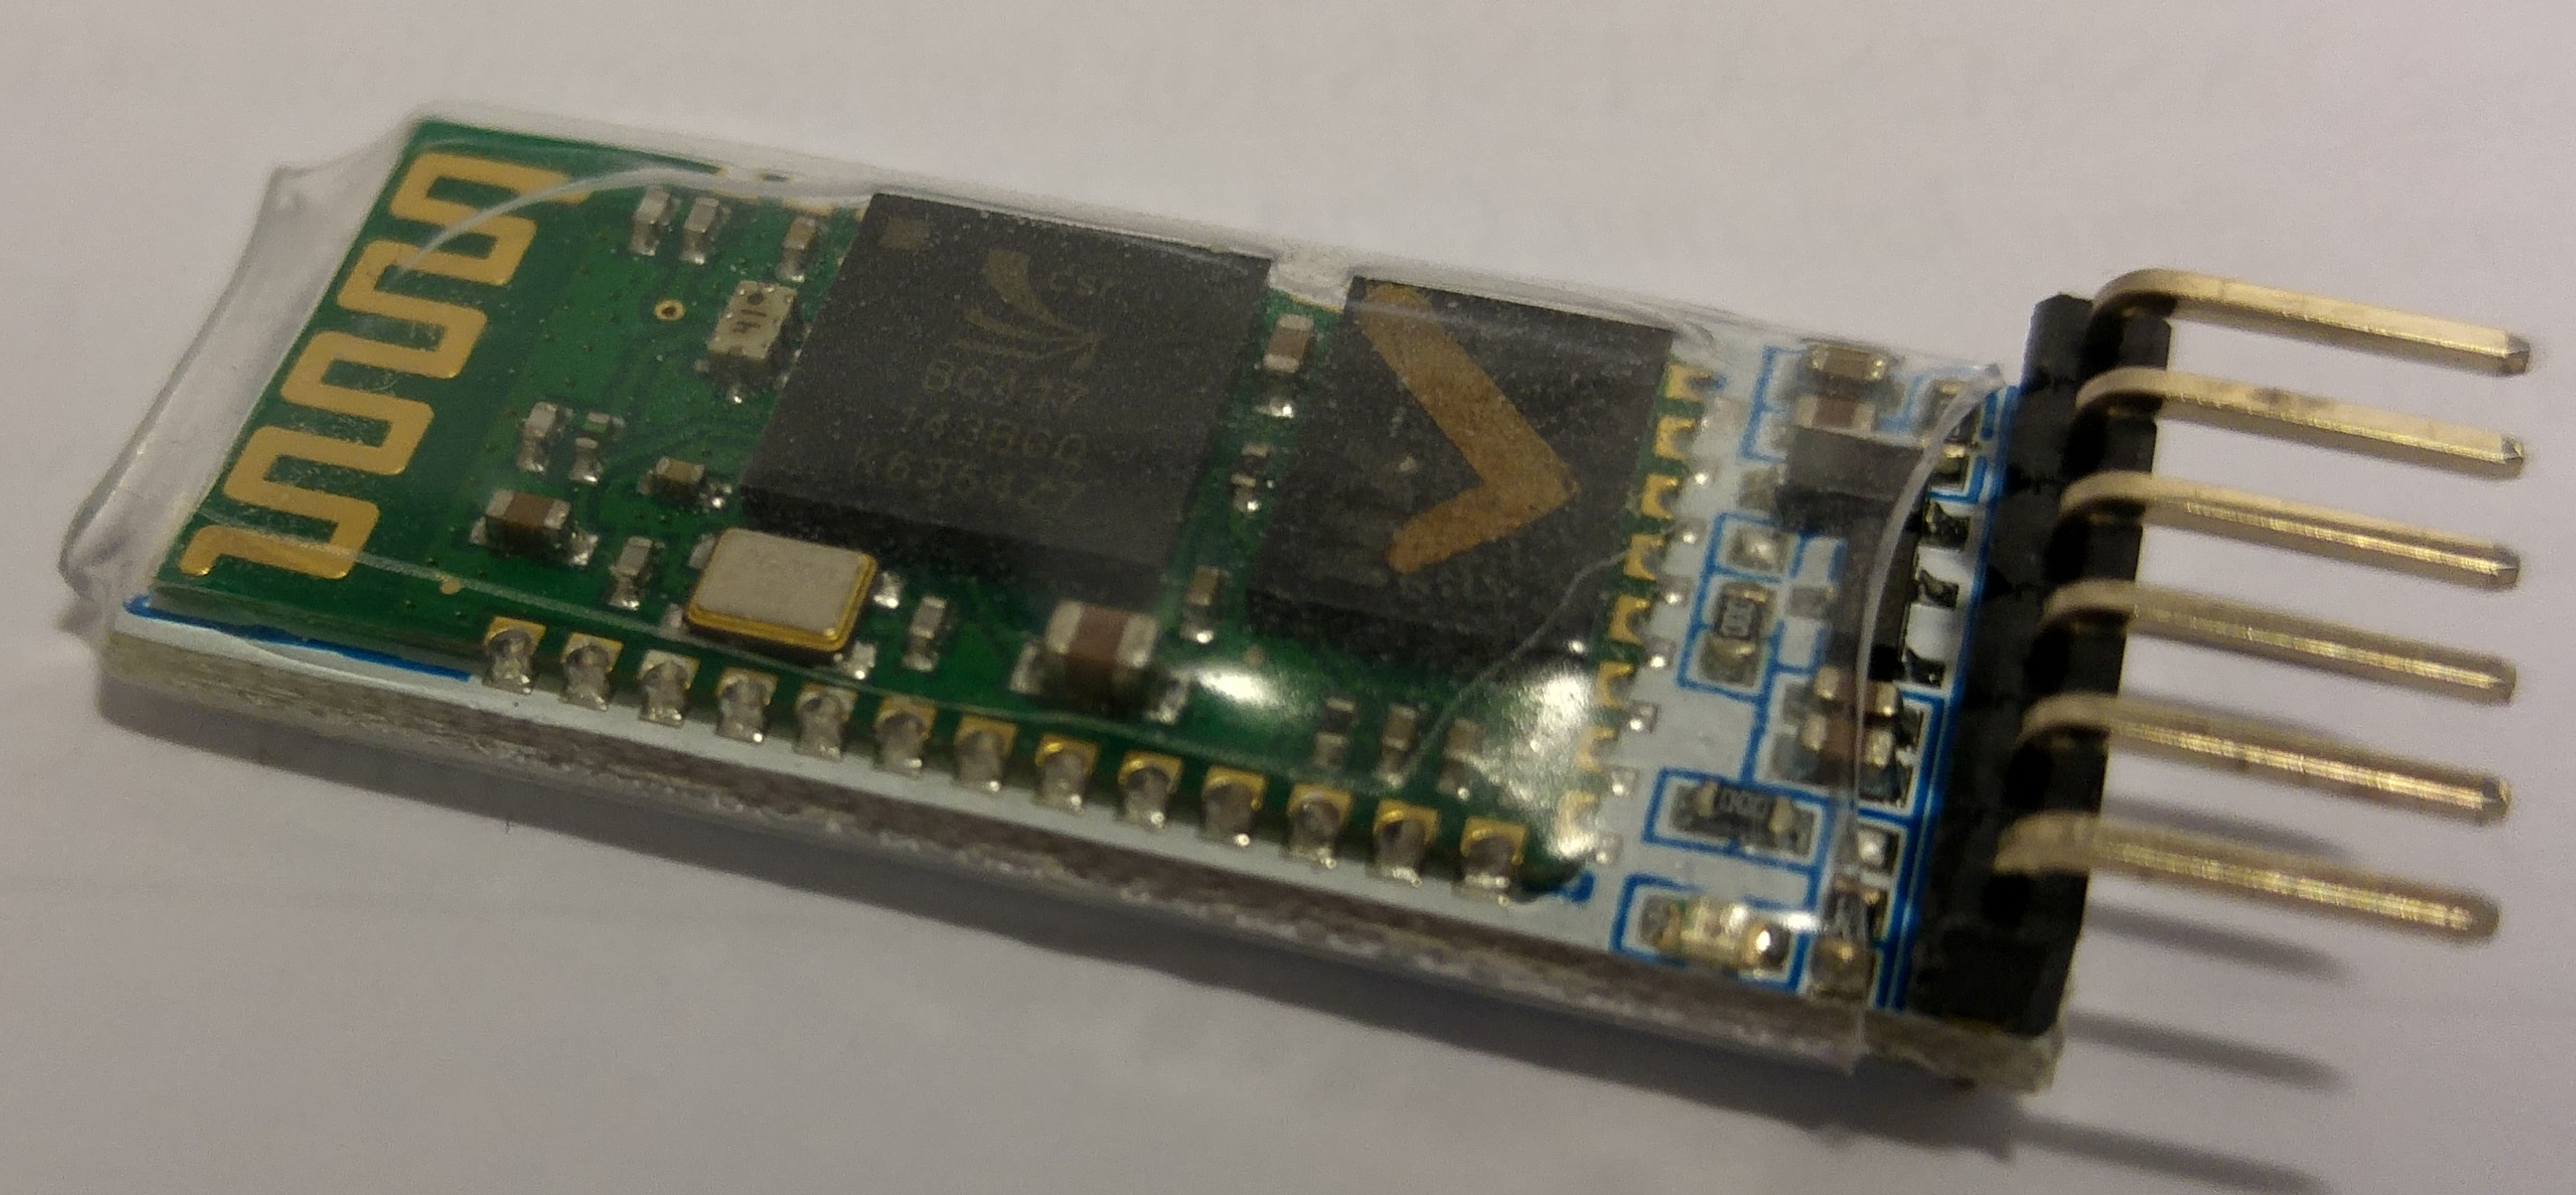
\includegraphics[width=0.5\textwidth]{HC05.jpg}
    \caption{The HC-05 chip for serial over Bluetooth. It costs roughly £4 and has a range of about 10m. Requiring a pin to pair the devices, it can have the role of either slave (wait for connection) or master (search for device to connect to).}
    \label{fig:HC-05}
\end{figure}


As Smart Agents, we used the Raspberry PI 3 - a single board computer. It has USB, Ethernet, WiFi and Bluetooth built in, enabling communication with the Edge Devices and the Cloud. Also popular for IoT applications due to its low price, the PI can run PC scale applications on its Linux operating system.

We used STFC's SCD Cloud which gave access to a virtual machine running Scientific Linux 7. A common LAN enabled communication with the Smart Agents.

% ✔ We used Arduino Unos (£25-30) as edge devices. They have X inputs and outputs (analog and digital) and can be loaded with pre-compiled programs.
% ✔ HC-05 chip for Bluetooth option (picture of HC-05, range=10m?, cost=£4...)
% ✔ Raspberry pi as smart agents. Stats – 1GB RAM, can be run headless, use linux...
% ✔ SCD Cloud machine (Scientific Linux 7) hugely useful, blah.

\subsection{Setup}

\begin{figure}
    \centering
    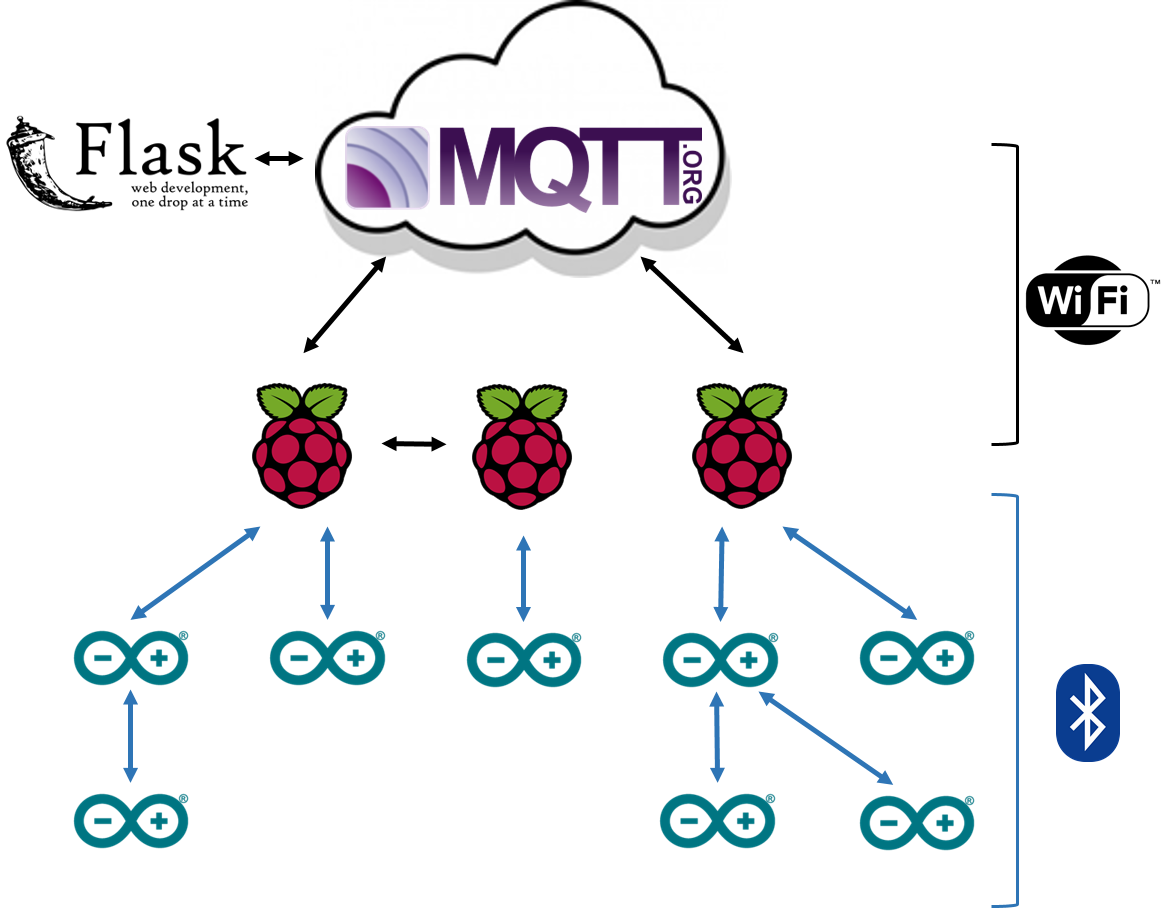
\includegraphics[width=0.5\textwidth]{Architecture.png}
    \caption{The architecture}
    \label{fig:architecture}
\end{figure}

The Cloud machine was setup as the MQTT broker using Mosquitto. There were three endpoints that communicate with the hub: Smart Agents, Broker Services and the web application. The Smart Agents interacted with the hub over TCP/IP using the Paho MQTT client library for Python. Each acted as a gateway to the Cloud for any connected Edge Devices. Broker Services ran on the Cloud as a Python script, also using Paho. Its purpose was to publish a list of currently connected devices for discovery. Using a Flask module - Flask-MQTT - a web application is served allowing a user to subscribe to topics for an overview of the data flows in the network. 

A Smart Agent can connect up to seven devices in a Bluetooth piconet. The agent scans for devices with a name matching a predefined address pattern, and then attempts to connect. However, each PI has a single Bluetooth chip so it cannot scan for devices and receive/send simultaneously. With scanning taking approximately twenty seconds, it was interrupting communication by introducing a delay. To counter this, we used a fixed list of devices to connect to which are always available making scanning unnecessary. While this seems restrictive, it works adequately for a variety of use cases - such as statically placed sensors in a house or vehicle controlled by a central smart agent. Alternatively, the same serial protocol can work over USB where scanning is almost instantaneous and Edge Devices can be connected or removed at will.


% Each edge device is identified by a unique ID which is a random number 
% ✔ Communication between Smart Agent and Edge via Bluetooth.
% What is Bluetooth /why is it a good option for communicating with low memory/power/connectivity devices? PAIRING!
% ✔ Smart agents run Piduino to interface between MQTT Pub/Sub and the inputs and outputs in the edge
% ✔ Broker (mosquitto) runs on cloud, as does telemetry and monitoring applications (broker services) and a flask app.
% Pretty diagrams and pictures of the equipment

% ✔ Diagram with the pretty logos on it I made for the pre-coffee talk. I’ll go find it. The programming
% Exact topic structure that we used
% Pretty graph of some data collected

\subsection{Data}
could record data from sensors on the Edge Devices, forward it to a Smart Agent that would handle publishing the data to the Cloud. The Cloud  

% Graph, and also some brief waffle about what’s on the graph.
% Picture of the Arduino/raspberry pi setup